% ----------------------------------------------------
% VARIABLES
% ----------------------------------------------------

\def \myPlace{FH JOANNEUM - University of Applied Sciences}
\def \myTitle{Dynamic Resource Allocation and Scaling of Stateful Workloads in
Kubernetes}
\def \mySubtitle{A Comparative Study of Reactive and Predictive Scaling Approaches for Redis Clusters}
\def \myStudy{Wirtschaftsinformatik}
\def \myName{Johann Krischan Hipolito}
\def \myAdvisor{Michael Nestler}
%\def \myExternalAdvisor{John Doe, PhD}
\def \myDate{Graz, 2026}

% ----------------------------------------------------
% PACKAGES
% ----------------------------------------------------

\documentclass[12pt,a4paper]{report}
\usepackage{listings}       % for \begin{lstlisting}
\lstset{
  breaklines=true,
  breakatwhitespace=true, % Optional: only breaks at spaces, keeping commands intact
  postbreak=\mbox{\textcolor{red}{$\hookrightarrow$}\space}, % Optional: adds a little arrow to show a line broke
  basicstyle=\linespread{0.9}\ttfamily\footnotesize,
}
\usepackage{acronym}        % for \ac{HPA}, \acp{CRD} etc.
\usepackage{siunitx} 
\usepackage[left=3.5cm, right=3cm, top=3cm, bottom=3cm]{geometry}
\usepackage{titlesec}
\usepackage{fancyhdr}
\usepackage{graphicx}
\usepackage{setspace}
\usepackage{tocloft}  % Für die Inhaltsverzeichnisformatierung
\usepackage{amsmath}
\usepackage{caption}
\usepackage[T1]{fontenc}
\usepackage[utf8]{inputenc}
\usepackage{pdfpages}
\usepackage[sfdefault]{carlito} % Ersatz für Calibri, sieht fast genau gleich aus
\usepackage{microtype}      % besseres Justieren, weniger Überhänge am Rand
\setlength{\emergencystretch}{3em} % letzter Ausweg: Zeile dehnen statt über den Rand laufen
\usepackage[backend=biber,style=apa,hyperref=true]{biblatex}
\usepackage{csquotes}
\usepackage{hyperref}

% ----------------------------------------------------
% SETTINGS
% ----------------------------------------------------

% Bibtex settings
\addbibresource{sources.bib}

% Entferne Einrückung im Inhaltsverzeichnis
\cftsetindents{section}{0em}{2em}   % Entfernt Einrückung für Sections
\cftsetindents{subsection}{2em}{2em} % Einrückung für Subsections (optional)
\cftsetindents{subsubsection}{4em}{2em} % Einrückung für Subsections (optional)

% Formatierung Inhaltsverzeichnis
\renewcommand{\cftsecdotsep}{\cftdotsep}
\renewcommand{\cftpartleader}{\cftdotfill{\cftdotsep}}
\renewcommand{\cftchapleader}{\cftdotfill{\cftdotsep}}
\renewcommand{\cftsecleader}{\cftdotfill{\cftdotsep}}
\renewcommand{\cftsubsecleader}{\cftdotfill{\cftdotsep}}

% Kopf- und Fußzeilen
\pagestyle{fancy}
\fancyhf{}
\fancyhead[L]{\nouppercase{\rightmark}} % \rightmark gibt die aktuelle Section wieder
\fancyfoot[C]{\thepage}

% Stil für Kopfzeile ausblenden
\fancypagestyle{nohead}{%
  \fancyhf{} % Kopf- und Fußzeile leeren
  \renewcommand{\headrulewidth}{0pt} % Kopfzeilenlinie entfernen
  \fancyfoot[C]{\thepage} % Seitennummer beibehalten
}

% Absatzformatierung
\setlength{\parskip}{6pt}
\setlength{\parindent}{0pt}

% Trennlinie für Fußnoten
\renewcommand{\footnoterule}{\rule{5cm}{0.4pt}\vspace{4pt}}

% Nummerierung der Sections ohne Kapitelnummer
\renewcommand{\thesection}{\arabic{section}}

\setcounter{tocdepth}{3}
\setcounter{secnumdepth}{3} % Subsubsections bekommen auch eine Nummer

% ----------------------------------------------------
% DOCUMENT
% ----------------------------------------------------

\setlength{\headheight}{14.49998pt}
\begin{document}

% Deckblatt
% ----------------------------------------------------
% Hier sollte nichts verändert werden außer bei Änderung der Sprache.
% Es gibt Variablen im main.tex File.
% ----------------------------------------------------

\begin{titlepage}

  \begin{center}

    % FH Joanneum Branding
    \bf{\myPlace}

    \vspace{2.0cm}

    % Titel der Arbeit
    \bf{\myTitle}

    % Untertitel der Arbeit
    \ifdef{\mySubtitle}{
      \bf{\mySubtitle}
    }{}

    \vspace{2.0cm}

    % Bachelorarbeit Beschreibung
    \bf{
      Bachelorarbeit

      zur Erlangung des akademischen Grades

      „Bachelor of Science in Engineering“

      eingereicht am Studiengang Wirtschaftsinformatik

      Studienrichtung: \myStudy
    }

    \vspace{2.0cm}

    % Autor:in
    \bf{Verfasst von: \myName}

    \vspace{2.0cm}

    % Betreuung
    \bf{Betreuung: \myAdvisor}

    % Externe Betreuung
    \ifdef{\myExternalAdvisor}{
      \bf{Firmenbetreuung: \myExternalAdvisor}
    }{
    }

    \vspace{2.0cm}

    % Ort und Datum
    \bf{\myDate}

    \vspace{2.0cm}

    % FH Joanneum Logo
    
\includegraphics[height=3cm]{assets/images/FH_LOGO}

  \end{center}

\end{titlepage}

%**********************************************************************


% Ab hier römische Seitenzahlen für Verzeichnisse
\pagenumbering{roman}
\pagestyle{plain}

% Sperrvermerk (keine Kopfzeile, keine Linie)
%\newpage
%\phantomsection
%\section*{Sperrvermerk}
%\addcontentsline{toc}{section}{Sperrvermerk}
%Hier steht der Sperrvermerk.

% Ehrenwörtliche Erklärung (keine Kopfzeile, keine Linie)
\newpage
\phantomsection
\section*{Ehrenwörtliche Erklärung}
\addcontentsline{toc}{section}{Ehrenwörtliche Erklärung}
Hier steht die ehrenwörtliche Erklärung.

% Danksagung/Widmung (keine Kopfzeile, aber Fußzeile mit Seitenzahl)
%\newpage
%\phantomsection
%\section*{Danksagung/Widmung}
%\addcontentsline{toc}{section}{Danksagung/Widmung}
%Hier kann die Danksagung oder Widmung stehen.

% Inhaltsverzeichnis
\newpage
\pagestyle{empty}
\renewcommand{\contentsname}{} % Entfernt die Standardüberschrift
\phantomsection
\section*{Table of Contents}
\addcontentsline{toc}{section}{Table of Contents} % Fügt zum Inhaltsverzeichnis hinzu
\vspace{-3cm} % Abstand verringern
\tableofcontents
\newpage

% Abbildungsverzeichnis
\newpage
\pagestyle{empty}
\renewcommand{\listfigurename}{} % Entfernt die Standardüberschrift
\phantomsection
\section*{List of Figures}
\addcontentsline{toc}{section}{List of Figures} % Fügt zum Inhaltsverzeichnis hinzu
\vspace{-1.5cm} % Abstand verringern
\listoffigures
\newpage

% Tabellenverzeichnis
\newpage
\pagestyle{empty}
\renewcommand{\listtablename}{} % Entfernt die Standardüberschrift
\phantomsection
\section*{List of Tables}
\addcontentsline{toc}{section}{List of Tables}
\vspace{-1.5cm} % Abstand verringern
\listoftables
\newpage

% Abkürzungsverzeichnis (keine Kopfzeile, keine Linie)
\newpage
\pagestyle{fancy} % Hier wieder auf fancy stellen, um Seitenzahlen zu zeigen
\fancyhead{}
\renewcommand{\headrulewidth}{0pt}  % Entfernt die Linie in der Kopfzeile
\phantomsection
\section*{List of Abbreviations}
\addcontentsline{toc}{section}{List of Abbreviations}
\begin{acronym}[YAML]   % longest acronym goes in brackets for alignment
    \acro{API}{Application Programming Interface}
    \acro{YAML}{YAML Ain't Markup Language}
    \acro{KEDA}{Kubernetes Event-Driven Autoscaling}
    \acro{CRD}{Custom Resource Definition}
    \acro{HTTP}{Hypertext Transfer Protocol}
    \acro{HPA}{Horizontal Pod Autoscalar}
\end{acronym}

% Symbolverzeichnis (keine Kopfzeile, keine Linie)
\newpage
\phantomsection
\section*{List of Symbols}
\addcontentsline{toc}{section}{List of Symbols}
Hier steht das Symbolverzeichnis.

% Formelverzeichnis (keine Kopfzeile, keine Linie)
\newpage
\phantomsection
\section*{List of Formulas}
\addcontentsline{toc}{section}{List of Formulas}
Hier steht das Formelverzeichnis.


% Kurzfassung und Abstract (keine Kopfzeile, keine Linie)
\newpage
\phantomsection
\section*{Kurzfassung}
\addcontentsline{toc}{section}{Kurzfassung}
Die Migration zustandsbehafteter Workloads, wie etwa partitionierter Datenbanken wie Redis, nach Kubernetes verursacht erhebliche architektonische Konflikte. Native Kubernetes-Skalierungsmechanismen, insbesondere der Horizontal Pod Autoscaler (HPA) und der \texttt{StatefulSet}-Controller, gehen von der generellen Austauschbarkeit von Rechenressourcen aus. Bei Scale-in-Vorgängen verwenden sie einen topologieblinden Löschmechanismus in umgekehrter Reihenfolge, der notwendige Datenmigrationsprotokolle umgeht und einen katastrophalen Datenverlust riskiert.

Diese Arbeit untersucht diese architektonischen Einschränkungen empirisch anhand eines deterministischen, lastfreien A/B-Tests. Die Studie evaluiert den Scale-in eines Redis-Clusters von vier auf drei Master-Knoten mit \num{5000} Datensätzen (Keys). Dabei wird die native HPA-Baseline mit dem Opstree Redis Operator, gesteuert durch Kubernetes Event-driven Autoscaling (KEDA), verglichen.

Die empirischen Ergebnisse zeigen, dass ein nativer HPA-Scale-in einen massiven Datenverlust verursacht. Dies führte zum sofortigen Verlust von 25\,\% des Datensatzes (\num{1250} Keys), \num{4096} verwaisten Hash-Slots und einer clusterweiten Nichtverfügbarkeit. Im Gegensatz dazu fing der Operator den Skalierungsbefehl erfolgreich ab, um einen präemptiven, topologiebewussten Resharding-Prozess zu orchestrieren. Dies ermöglichte einen reibungslosen Scale-in ohne Datenverlust und mit durchgehender Verfügbarkeit.

Letztendlich belegt diese Untersuchung, dass die Implementierung domänenspezifischer Orchestrierungslogik durch das Operator-Pattern nicht nur eine operative Erleichterung, sondern eine absolute architektonische Notwendigkeit darstellt, um die Datenintegrität bei der Skalierung zustandsbehafteter Workloads in Kubernetes zu gewährleisten.
\newpage
\phantomsection
\section*{Abstract}
\addcontentsline{toc}{section}{Abstract}
The migration of stateful workloads, such as sharded databases like Redis, into Kubernetes introduces significant architectural friction. Native Kubernetes scaling primitives, specifically the Horizontal Pod Autoscaler (HPA) and the \texttt{StatefulSet} controller, operate on the assumption of compute fungibility. During scale-in operations, they employ a topology-blind, reverse-ordinal pod deletion mechanism that bypasses necessary data migration protocols, risking catastrophic data loss.

This thesis empirically investigates these architectural limitations through a deterministic, quiescent A/B test. The study evaluates a scale-in operation from four to three master nodes on a Redis cluster containing \num{5000} keys. It compares the native HPA baseline against the Opstree Redis Operator, driven by Kubernetes Event-driven Autoscaling (KEDA).

The empirical findings demonstrate that a native HPA scale-in induces a severe data cliff. This resulted in the immediate loss of 25\% of the dataset (\num{1250} keys), \num{4096} orphaned hash slots, and cluster-wide unavailability. Conversely, the operator successfully intercepted the scaling command to orchestrate a pre-emptive, topology-aware resharding process. This achieved a graceful scale-in with zero data loss and continuous cluster availability.

Ultimately, this research proves that encoding domain-specific orchestration logic via the Operator pattern is not merely an operational convenience, but an absolute architectural necessity for safeguarding data integrity when scaling stateful workloads in Kubernetes.

% Nach dem Abstract auf arabische Seitenzahlen umstellen
\newpage
\pagenumbering{arabic}

% Ab hier eine Kopfzeile und eine Linie
\pagestyle{fancy}  % Ab der Einleitung mit Kopfzeile
\setcounter{section}{0}

\pagestyle{fancy}  % Kopfzeile und Linie wieder aktiv
\fancyhead[L]{\nouppercase{\rightmark}} % Kopfzeile mit aktueller Section
\renewcommand{\headrulewidth}{0.4pt}  % Setze die Linie in der Kopfzeile wieder auf 0.4pt

% Kapitel der Arbeit
\newpage
\section{Introduction}
\label{sec:introduction}

\subsection{Background}
\label{subsec:background}

\subsection{Problem Statement}
\label{subsec:problem-statement}

\subsection{Objectives}
\label{subsec:objectives}
\newpage
\section{Theoretical Foundations}
\label{sec:theoretical-foundations}

\subsection{Kubernetes Concepts Overview}
\label{subsec:kubernetes-concepts}

\subsubsection{Use Cases of Kubernetes}
\label{subsec:use-cases}

\subsection{Autoscaling in Kubernetes}
\label{subsec:autoscaling}

\subsection{Stateful vs. Stateless Workloads}
\label{subsec:stateful-vs-stateless}

\subsubsection{Problems with Stateful Workloads in Kubernetes}
\label{subsec:problems-stateful-workloads}

\subsection{Metrics and Observability in Kubernetes}
\label{subsec:metrics-observability}
\newpage
\section{Related Works into Kubernetes Autoscaling with Stateful Workloads}
\label{sec:related-work}

\subsection{Existing Research into Stateful Kubernetes Autoscaling}
\label{subsec:existing-research}

\subsection{Industry Implementations and Best Practices}
\label{subsec:industry-best-practices}

\subsection{Research Gaps in Current Research and Opportunities for Improvement}
\label{subsec:research-gaps}
\newpage
\section{Methodology and Experimental Setup}
\label{sec:methodology-and-experimental-setup}

\subsection{Experimental Setup}
\label{subsec:setup}

\begin{figure}[htbp]
    \centering
    \caption{High-level architecture overview of the experimental setup.}
    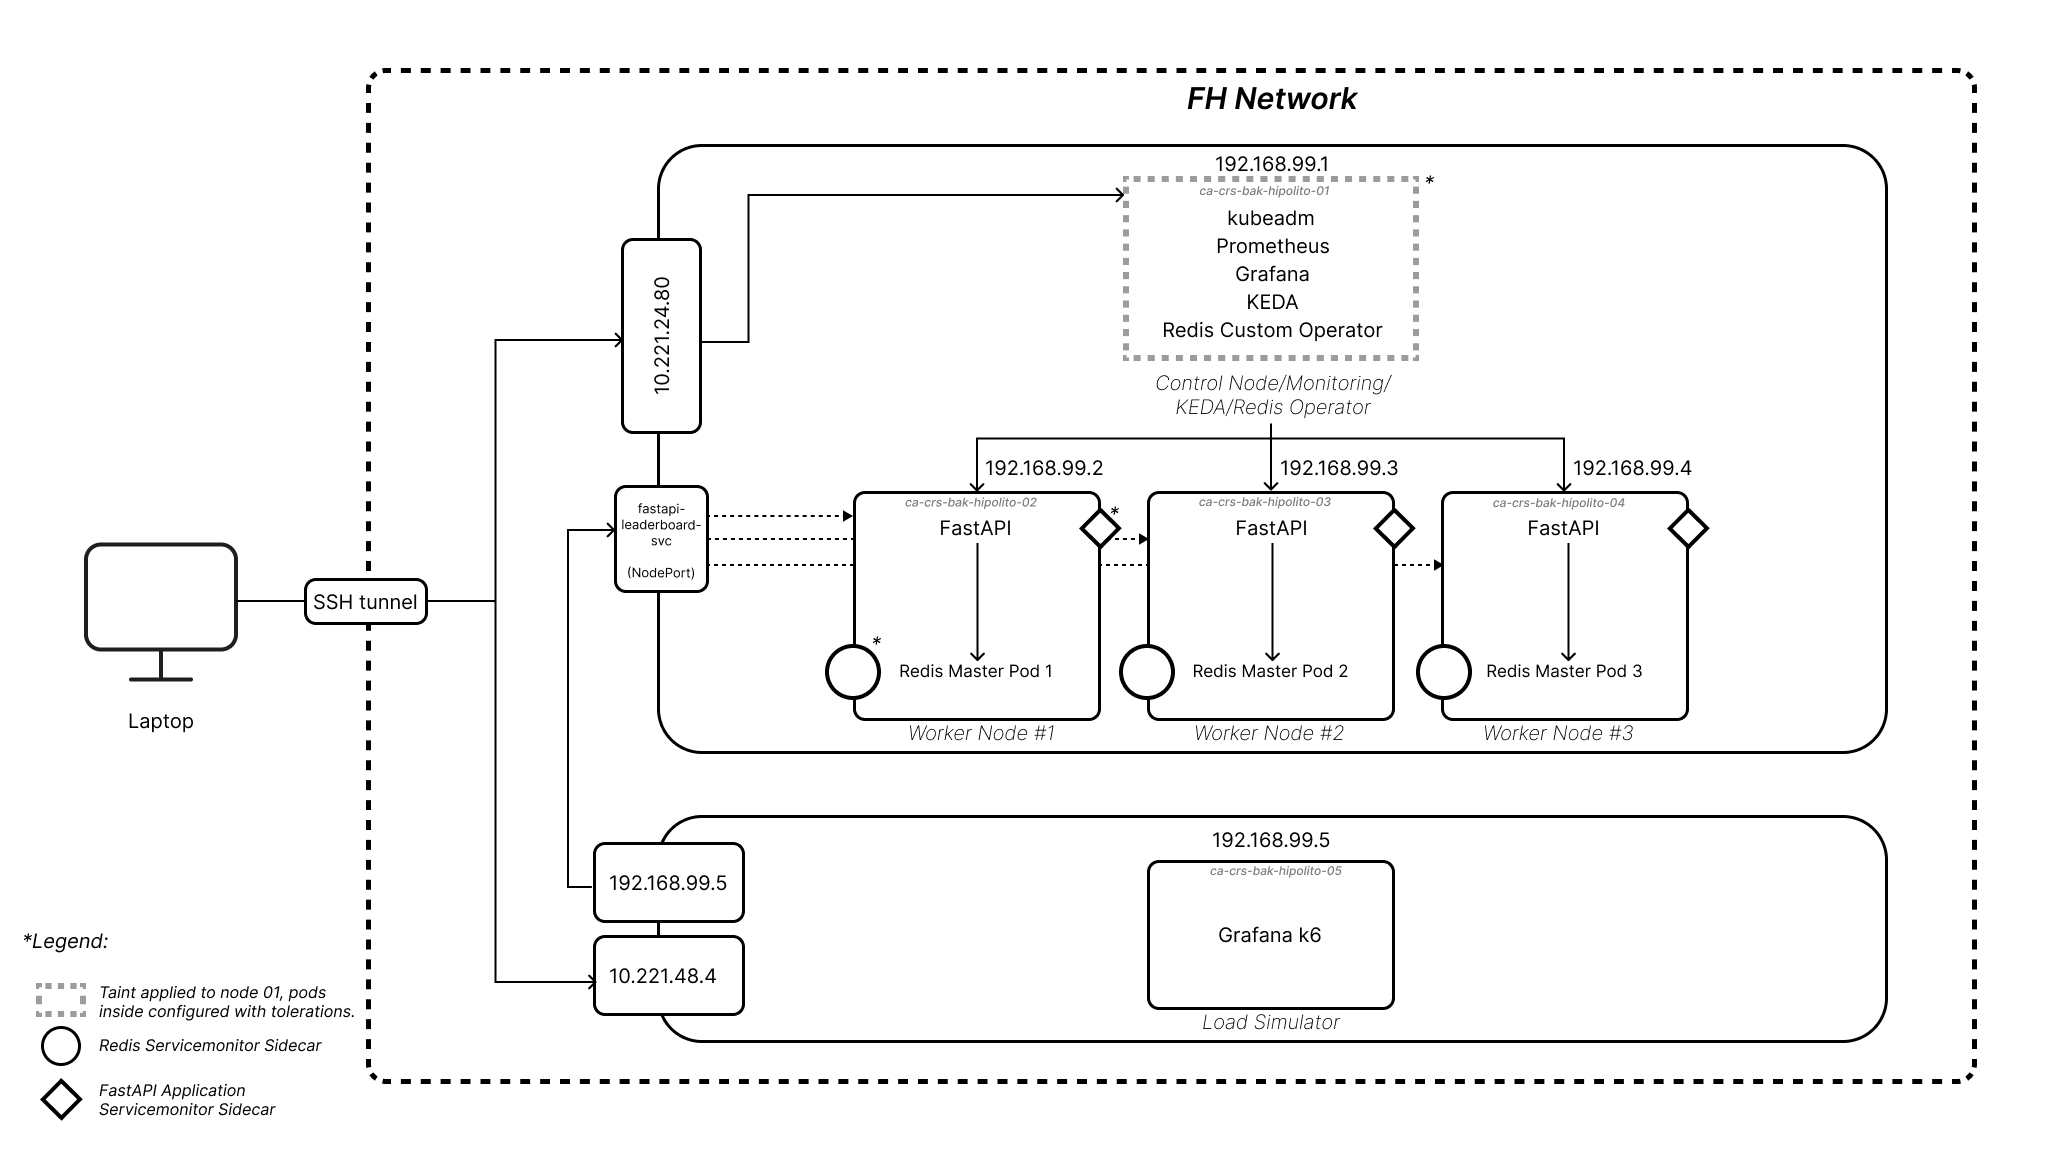
\includegraphics[angle=90,height=\textheight]{assets/images/high-level-architecture-overview-graph.png}
    \label{fig:arch-overview}
\end{figure}

\subsubsection{Virtualisation Environment}
\label{subsubsec:ve}

\subsubsection{Routing}
\label{subsubsec:routing}

\subsubsection{Redis Cluster Configuration}
\label{subsubsec:redis-cluster-configuration}

\subsubsection{FastAPI Application Design}
\label{subsubsec:fastapi-application-design}

\subsection{Autoscaling Configuration}
\label{subsec:autoscaling-configuration}

\subsection{Load Simulation}
\label{subsec:load-simulation}

\subsection{Evaluation Metrics and Data Collection}
\label{subsec:evaluation-metrics-and-data-collection}

\newpage
\section{Results and Analysis}
\label{sec:results-and-analysis}

\subsection{Compute and Memory Saturation}
\label{subsec:compute-memory}

\subsection{Network and Data Pipeline}
\label{subsec:network-data-pipeline}

\subsection{Application Throughput and Reliability}
\label{subsec:application-throughput-reliability}

\subsection{Final Comparison between Reactive Scaling and Predictive Scaling}
\label{subsec:final-comparison}

\newpage
\section{Conclusion}
\label{sec:conclusion}

\subsection{Summary of Findings}
\label{subsec:summary}

\subsection{Discussion}
\label{subsec:discussion}

\newpage
\appendix

% Anhang (keine Kopfzeile, keine Linie)
\pagestyle{nohead} % Kopfzeile nur auf dieser Seite ausblenden
\phantomsection
\section*{Appendix}
\addcontentsline{toc}{section}{Appendix}

% \subsection*{Appendix A: Test Execution Script}
% \begin{lstlisting}[language=bash, caption={The deterministic data-safety experiment script (data-safety-experiment.sh).}]

% Glossar (keine Kopfzeile, keine Linie)
\newpage
\pagestyle{nohead} % Kopfzeile nur auf dieser Seite ausblenden
\phantomsection
\section*{Glossar}
\addcontentsline{toc}{section}{Glossary}\begin{description}

    \item[ConfigEpoch] A collision-resolution concept in a Redis Cluster used to determine which node holds the authoritative claim over a specific hash slot during split-brain or network partition events.
    
    \item[CRD (Custom Resource Definition)] An API extension mechanism in Kubernetes that allows users to define and instantiate custom resources, such as the \texttt{RedisCluster} resource utilized by the Opstree operator.
    
    \item[Data Cliff] A term utilized in this thesis to describe the sudden, catastrophic loss of data and cluster availability that occurs when a stateful node is terminated without prior data migration.
    
    \item[Ghost Pod] A pod provisioned by a generic autoscaler (like HPA) that joins a Kubernetes \texttt{StatefulSet} but remains unintegrated into the database topology, meaning it holds zero hash slots and serves no traffic.
    
    \item[Hash Slot] The fundamental unit of data partitioning in a Redis Cluster. The total keyspace is divided into exactly \num{16384} hash slots, which must be distributed across the master nodes to maintain cluster availability.
    
    \item[Horizontal Pod Autoscaler (HPA)] A native Kubernetes control loop that automatically updates a workload resource (such as a \texttt{StatefulSet}) to match demand based on observed metrics, such as average CPU utilization.
    
    \item[KEDA (Kubernetes Event-driven Autoscaling)] A single-purpose, lightweight component added to a Kubernetes cluster to drive autoscaling based on external event metrics, such as Prometheus cache-miss ratios.
    
    \item[Operator Pattern] A software extension to Kubernetes that encodes domain-specific operational knowledge into a custom controller to automate the lifecycle and topology management of complex stateful applications.
    
    \item[Quiescent] A state of execution where no external read or write traffic is applied to the database. This state is used in the experimental methodology to isolate scaling mechanics from load-induced resharding interruptions.
    
    \item[Resharding] The process of live-migrating hash slots, along with the underlying data they contain, from one node to another within an active database cluster.
    
    \item[Stateful Workload] An application or database (such as Redis) that persists client data across sessions, meaning its underlying compute pods contain unique data and are not strictly interchangeable.
    
    \item[StatefulSet] A native Kubernetes workload API object used to manage stateful applications, providing strict guarantees about the ordering and uniqueness of a set of Pods, including the enforcement of reverse-ordinal deletion during scale-in operations.

\end{description}


% Literaturverzeichnis (keine Kopfzeile, keine Linie)
\newpage
\pagestyle{nohead} % Kopfzeile nur auf dieser Seite ausblenden
\phantomsection
\section*{List of References}
\addcontentsline{toc}{section}{List of References}
\printbibliography[heading=none]

% Stichwortverzeichnis (keine Kopfzeile, keine Linie)
%\newpage
%\thispagestyle{nohead} % Kopfzeile nur auf dieser Seite ausblenden
%\phantomsection
%\section*{Stichwortverzeichnis}
%\addcontentsline{toc}{section}{Stichwortverzeichnis}
%Hier steht das Stichwortverzeichnis.

% Anlagen (keine Kopfzeile, keine Linie)
\newpage
\thispagestyle{nohead} % Kopfzeile nur auf dieser Seite ausblenden
\phantomsection
\section*{Attachments}
\addcontentsline{toc}{section}{Attachments}
The following Attachments are included as a digital supplement to this thesis (as a ZIP archive in the submission system) and reference the complete codebase used for conducting the experiments.

\begin{description}

    \item[Attachment 1: Project repository (Quellcode)] \hfill \\
    The complete GitHub repository contains all Kubernetes manifests, Bash automation scripts (\texttt{data-safety-experiment.sh}), FastAPI deployment files, and the raw Markdown output logs of the conducted experiments. \\
    \textbf{URL:} \url{https://github.com/gitbudy360/bac-johann-hipolito} \\
    \textbf{Commit-Hash:} \texttt{be45110ff64e3f3a5527c91c6eba6a5c7270d18a}

    \item[Attachment 2: Grafana Dashboards] \hfill \\
    The \ac{JSON}-exports of the Grafana dashboards used for visualizing hash slot assignments and key metrics during the scale-in phases. Located in the \texttt{/k8s-cluster/grafana/} directory.

\end{description}

\end{document}

% ----------------------------------------------------
% Diese Vorlage wurde von Vanessa Reiter und Andreas Feichtinger erstellt.
% Anpassung für die Bachelorarbeit von Georg Mittenecker
% ----------------------------------------------------